\colorbox{yellow}{Denne delen er mye preget av ``vi``. Setningene bør bygges opp som ``Det ble ..``}

\subsection{Bildegjenkjenning}

Kongsberg anbefalte oss å bruke OpenCV, et åpen kildekode programvarebibliotek som brukes til bearbeiding av bilder og video. I tillegg ble vi oppfordret til å implementere programvaren i programmeringsspråket Matlab, siden Kongsberg internt bruker Matlab til prototyping. Flere på gruppa hadde erfaring med Matlab fra før, og vi så på dette som en god avgjørelse.

Da vi begynte prosjektet var siste stabile utgivelse av OpenCV versjon 2.4.8, som ikke støttet programmering i Matlab. For å bruke Matlab og OpenCV sammen hadde vi da to alternativer. Versjon 3.0 av OpenCV, som var under utvikling, støtter Matlab. Dessuten fantes det et tredjeparts kompatibilitetslag, \emph{mexopencv}, som gjorde det mulig å programmere med OpenCV i Matlab. Vi forsøkte begge muligheter. \emph{mexopencv} var vanskelig å kompilere på de ulike kombinasjonene av operativsystem og Matlab-versjon de ulike gruppemedlemmene satt med. Etter å ha kompilert det fikk vi dessuten problemer med at enkelte av grafikkortene vi brukte ikke var støttet av \emph{mexopencv}. Utviklingsversjonen av OpenCV, på sin side, fikk vi overhodet ikke kompilert. Antakelig skyldes dette at kodebasen for denne versjonen var under rask utvikling og dermed ustabil.

Etter å ikke ha fått Matlab og OpenCV til å fungere sammen, valgte vi å gå for en løsning der vi i stedet for Matlab implementerte programvaren for bildegjenkjenning i C++. Vi informerte Kongsberg om dette, og de var enige i at det var en god løsning. Etter å ha skiftet språk til C++, kom vi raskt igang med utviklingen og innen få dager hadde vi utviklet en enkel løsning for bildegjenkjenning.

\subsubsection{Innhenting av bilde og konvertering}

Fra kamera fikk vi et bilde i fargespekteret RGB\footnote{Red, Green, Blue}, som er lite egnet til å separere ulike farger fra hverandre. Vi valgte dermed å heller benytte fargespekteret HSV\footnote{Hue, Saturation, Value}, som er hyppig brukt innen bildeprosessering. Den første implementasjonen av gjenkjenningen baserte seg på å konvertere hvert bilde i videoen fra RGB, se figur [\ref{fig:firstiterationrgb}], til HSV, som vist i figur [\ref{fig:firstiterationhsv}].

\begin{figure}[h!]
	\centering
	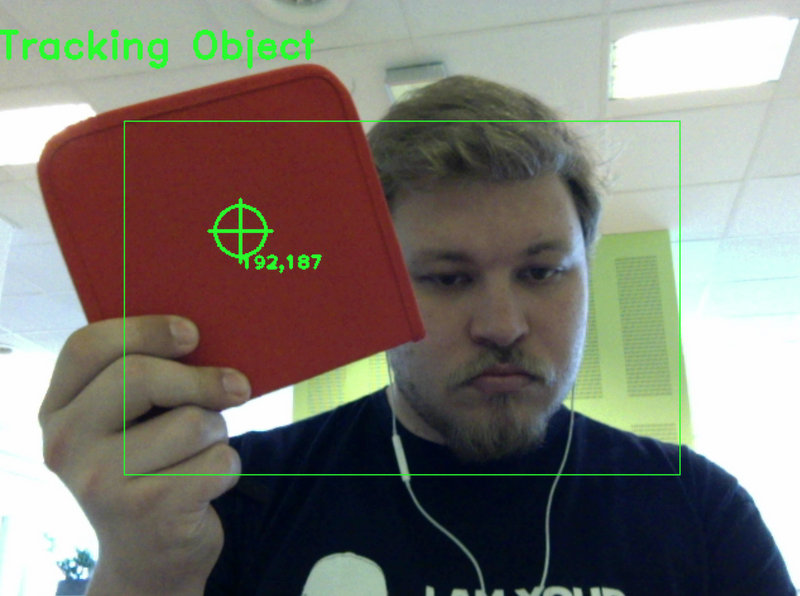
\includegraphics[scale=0.47]{img/first-rgb.jpg}
	\caption[Første iterasjon RGB bilde]{Bilde fra video i vanlig RGB}
	\label{fig:firstiterationrgb}
\end{figure}

\begin{figure}[h!]
	\centering
	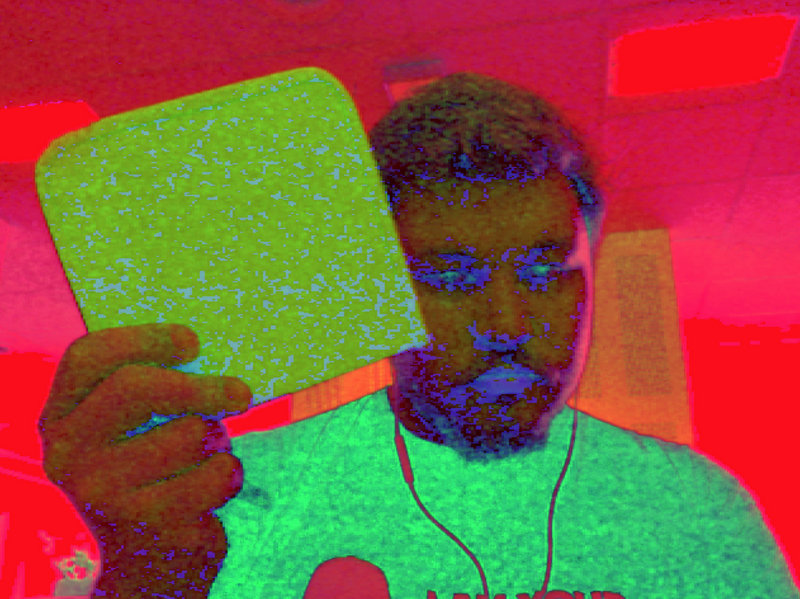
\includegraphics[scale=0.47]{img/first-hsv.jpg}
	\caption[Første iterasjon HSV bilde]{Bilde fra video konvertert til HSV}	\label{fig:firstiterationhsv}
\end{figure}

HSV baserer seg ikke på blanding av ulike farger, som RGB, men bruker nyanse, metningsgrad og lysverdi til å definere hver farge. Å konvertere bildet fra RGB til HSV gjør jobben med å peke ut en spesifikk farge lettere, og gjør det lettere å skille objekter fra andre. Et eksempel på et problem ved å bruke RGB er at dersom et objekt blir flyttet fra lys til skygge, endrer ikke RGB-verdiene seg langs én akse, men derimot på både R-, G- og B-aksene på en måte som er vanskelig å forutse. HSV oppfører seg mer forutsigbart -- i dette eksempelet endrer fargeverdien seg hovedsakelig i V-aksen.

\subsubsection{Deteksjon}

Etter å ha konvertert bildet til HSV, behandlet vi bildematrisen med et filter, som vi manuelt stilte inn med maksimum- og minimumverdier for \emph{hue}, \emph{saturation} og \emph{value}, vist i figur [\ref{fig:sliders}]. Vi satt da igjen med et binært bilde, der fargene som lå mellom disse maksimums- og minimumsverdiene er gjengitt i hvitt, mens alle andre farger er gjengitt i svart, som vist i figur [\ref{fig:firstiterationbinary}].

\begin{figure}[h!]
	\centering
	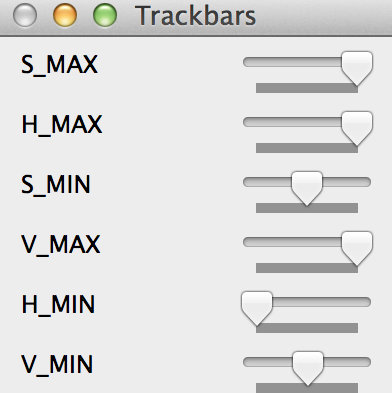
\includegraphics[scale=0.45]{img/sliders.jpg}
	\caption{Slidere for å velge HSV verdier}
	\label{fig:sliders}
\end{figure}

\begin{figure}[h!]
	\centering
	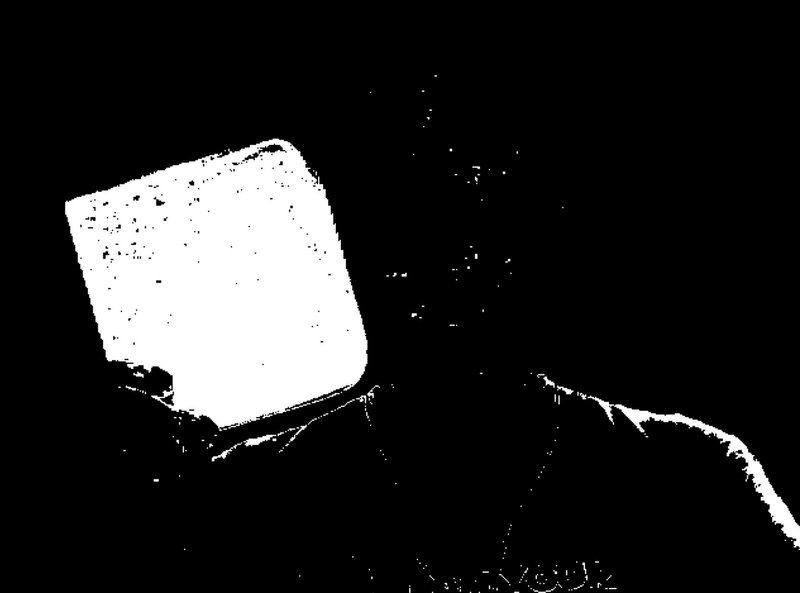
\includegraphics[scale=0.45]{img/first-binary.jpg}
	\caption[Første iterasjon binært bilde]{Resultatet av filtrering av et bilde før smoothing}
	\label{fig:firstiterationbinary}
\end{figure}

Nå som vi hadde et binært bilde, var det neste steget å velge ut ett objekt fra bildet slik at det kunne trackes. Med objekt menes her et sammenhengende hvitt område i det binære bildet. Algoritmen vår valgte ut det største objektet, og returnerte objektets midtpunkt. Dersom det var for mye støy i bildet, det vil si for mange ulike objekter, returnerte algoritmen ikke et punkt.

\subsubsection{Smoothing}

I det første steget klarte vi å fange opp et objekt, men som man kan se i figur [\ref{fig:firstiterationbinary}] er det mye støy i bildet. Vi implementerte derfor en smoothingalgoritme som gikk over det binære bildet og fjernet mindre ansamlinger med punkter og fremhevet de som var større. Dette førte til at vi fikk et renere bilde, med færre og tydeligere objekter. Resultatet av smoothingen kan man se i figur [\ref{fig:seconditerationbinary}].

\begin{figure}[h!]
	\centering
	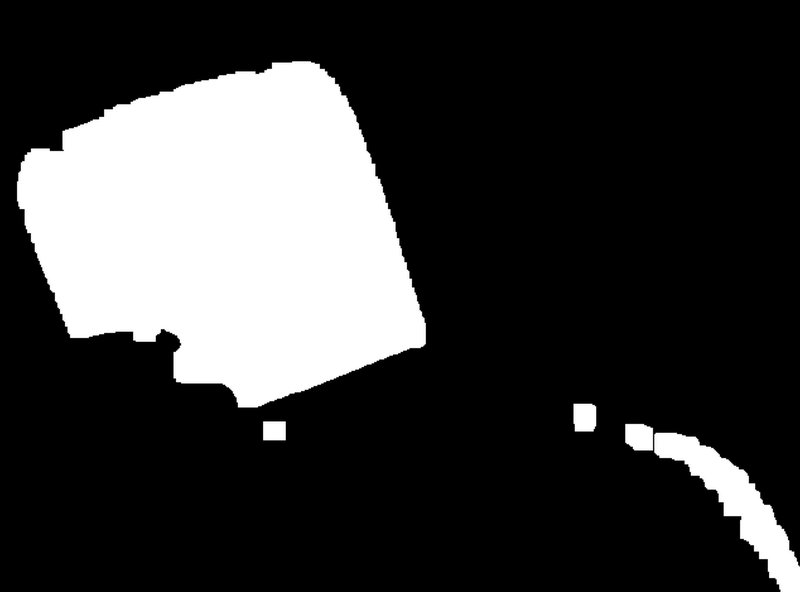
\includegraphics[scale=0.45]{img/second-binary.jpg}
	\caption[Andre iterasjon binært bilde]{Resultatet av filtrering av et bilde etter smoothing}
	\label{fig:seconditerationbinary}
\end{figure}

Smoothingen fremhevet de store objektene i bildet. Dette gjorde det betydelig lettere å fange opp kun det objektet vi var ute etter å følge, gitt riktig innstilling av fargefilterne, fordi små objekter i bildet med samme farge som objektet vi ville følge ble fjernet.

\subsubsection{Brukergrensesnitt}

Etter at vi hadde jobbet en del med systemet fant vi ut at det var tungvindt å hver gang manuelt stille inn hvilke farger som skulle følges ved hjelp av sliderne. Løsningen ble da at vi implementerte et enkelt kommandolinjegrensesnitt, der vi ved hjelp av kommandoen \texttt{center} kunne be programmet om å følge etter fargen som befant seg i sentrum av bildet. Grensesnittet er vist i figur [\ref{fig:commandmenu}]. Etter hvert som vi la til flere funksjoner i programmet, utvidet vi kommandolinjegrensesnittet med flere kommandoer.

\begin{figure}[h!]
	\centering
	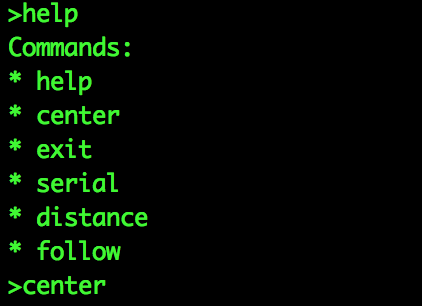
\includegraphics[scale=0.8]{img/command-menu.png}
	\caption{En oversikt over de tilgjengelige kommandoene i kommandolinjegrensesnittet}
	\label{fig:commandmenu}
\end{figure}

For å gjøre det enklere å følge spesifikke objekter i kamerabildet, implementerte vi senere en funksjon som lot oss klikke på objekter i bildet for å følge dem. Både denne funksjonaliteten og \texttt{center}-kommandoen fungerte slik at fargeverdien til punktet som var i sentrum av bildet eller som ble klikket på ble hentet inn, og at sliderne automatisk ble satt til denne verdien pluss/minus en margverdi. Gode margverdier ble funnet eksperimentelt, og vi kom fram til at en marg på $20$ eller $30$ for hver av aksene \emph{hue}, \emph{saturation} og \emph{value} fungerte godt i de fleste situasjoner.

\subsection{Valg av hardware}
\subsubsection{Første test med Arduino}
Det ble først bestemt at Arduino Uno skulle brukes til formålet. Fordelen var at det finnes et standard bibliotek for servoer. I utgangspunktet skulle systemet ha et gyrometer som skulle måle orienteringen av riggen og kompensere for dette. Slik at kameraet vill stå vinkelrett uansett hvordan flyet beveger seg. Det ble valgt å benytte seg av en modifsert utgave av biblioteket [\ref{GyroLib}]. Dette viste seg å bli et problem da Arduino ikke støtter multithreading. Det ble konflikt mellom PWM-delen av servobiblioteket og $U^2C$ som gyrometeret benytter seg av.

For å løse dette, ble det gjort forsøk på å benytte seg av to arduinoer. Lesingen av gyrometeret og pådrag til servoene skulle bli gjort på hver sin. UART ble benyttet som kommunikasjonsprotokoll mellom dem. Erfaringene viste at arduinoen som skulle motta kommandoer mottok mye støy. Pådraget til servoene ble dermed veldig ustabile. 

\subsubsection{Raspberry Pi}
Et alternativ til Arduino, var å bruke Raspberry Pi. Som presisert i "chapter ett eller annet (ref)", har Raspberry Pi multithreading. En lignende konflikt mellom pwm og I2c vil dermed ikke skje. Men det oppsto utfordringer da Raspberry Pi kun har 1 PWM-port. Det finnes en rekke biblioteker som løser dette ved å genere PWM-signal i software og sende dem gjennom en vanlig digital port. Til dette formålet ble biblioteket WiringPi[\ref{RaspLib}] benyttet. For gyromteret, ble et standard I2C-bibliotek brukt. 

Det viste seg at konfigurasjonen av WiringPi-biblioteket var tidkrevende, og det ble bestemt å gå tilbake til Arduino, men uten gyrometer.  

\subsubsection{Andre test med Ardunino}
Denne implimentasjonen består av en Arduino som kjører servobilioteket. Arduinoen får innput fra PC via USB, og gir pådrag til servoene basert på disse. Testene viste at servoene hadde en stabil oppførsel, og valget falt da på denne implementasjonen.   

\subsection{Konstruksjon av riggen}

\subsubsection{Planlegging}
Riggens oppgave er å endre synsretningen til kameraet etter kommando fra bildegjennkjenningen. Synsvinkelen kan modeleres som en vektor, hvor retningen til vektoren er variabel. Hvis vektoren, $\bf{v}$, settes inn i et koordinatsystem med utspring i origo og sfæriske koordinater, kan situasjonen beskrives som i figur [\ref{fig:spher}]

\begin{figure}[h!]
	\centering
	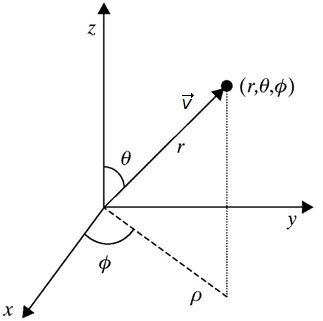
\includegraphics[scale=0.5]{img/RettVek.jpg}
	\caption{Sfærisk koordinatsystem}
	\label{fig:spher}
\end{figure}

hvor $\phi$ er vinkelen mellom x- og y-aksene og $\theta$ er vinkelen mellom z-aksen og xy-planet. Siden riggen skal festes til et fly og kameraet skal se ned på bakken vil det ikke være behov for vinkelretningen å bevege seg inn i den øvre halvdelen av koordinatsystemet. Det betyr at $\phi$ og $\theta$ kun trenger 180 graders utsving for å dekke hele den nedre halvdelen. Dermed kan hele dette omerådet dekkes ved hjelp av to servomotorer med 180 graders utslag satt sammen som i figur [\ref{fig:IdeRigg}]. 

\begin{figure}[h!]
	\centering
	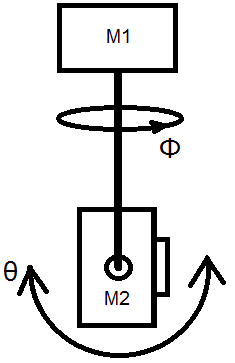
\includegraphics[scale=0.5]{img/BasicRiggIde.png}
	\caption{Servostyring av $\theta$ og $\phi$}
	\label{fig:IdeRigg}
\end{figure}

Hvor kameraet festes til servomotor 2 som beveger seg i retning $\theta$, mens servomotor 1 beverger servo2 og kamera i retning $\phi$. For å kunne trekke riggen inn i flyet ved landing ble det bestemt å feste riggen på en bom som kunne heves å senkes ved hjelp av en servomotor som vist i figur [\ref{fig:bom}].

\begin{figure}[h!]
	\centering
	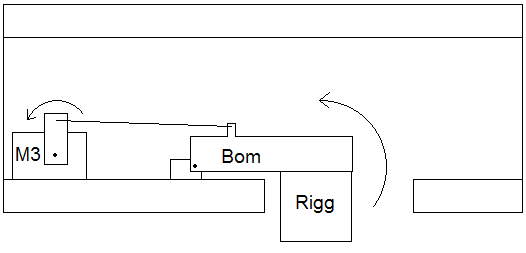
\includegraphics[scale=0.5]{img/Motor3.png}
	\caption{Servomotor 3 kan heve riggen inn i flykroppen.}
	\label{fig:bom}
\end{figure}


\subsubsection{Sammenstilling}
Riggen ble sammenstilt med målene på prototypeflyet til kongsberg som utgangspunkt [\textcolor{red}{Referere til PowerPoint}]. Med disse målene ble det klart at servomotorene måtte være små i størrelse og valget falt på servomotoren HD-1600A. Med sine beskjedene fysiske mål på 21.3x11.6x22.8 mm og en vekt på 6g \cite{PowerHD}, ble HD-1600A ansett som perfekt for dette formålet. HS-50 fra Hitec ble også vurdert, men med lavere dreimoment og betydelig høyere pris ble HD-1600A regnet som et bedre alternativ. For å bygge delene som skulle koble servoene sammen ble det brukt 6mm MDF plater fordi disse er stive og relativt sterke. Dette fører til at de ikke bøyes eller gir etter ved raske rotasjoner. Figur [\ref{fig:RiggTegn}] viser hvordan servomotorene er koblet sammen og figur [\ref{fig:RiggBilde}] viser et bilde av den ferdige prototype riggen. 

\begin{figure}[h!]
	\centering
	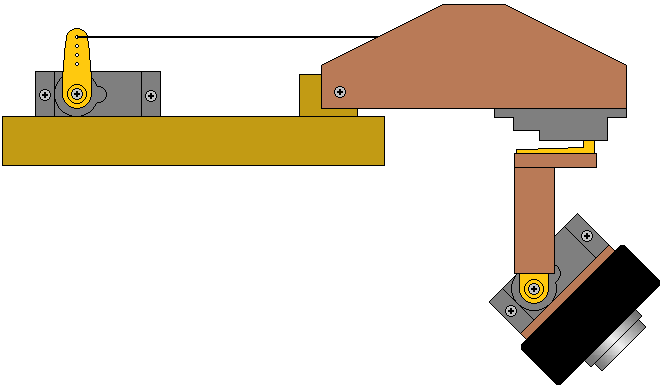
\includegraphics[scale=0.5]{img/RIGG_sattsammen.png}
	\caption{Tegning av mekaniske rigg}
	\label{fig:RiggTegn}
\end{figure}

\begin{figure}[h!]
	\centering
	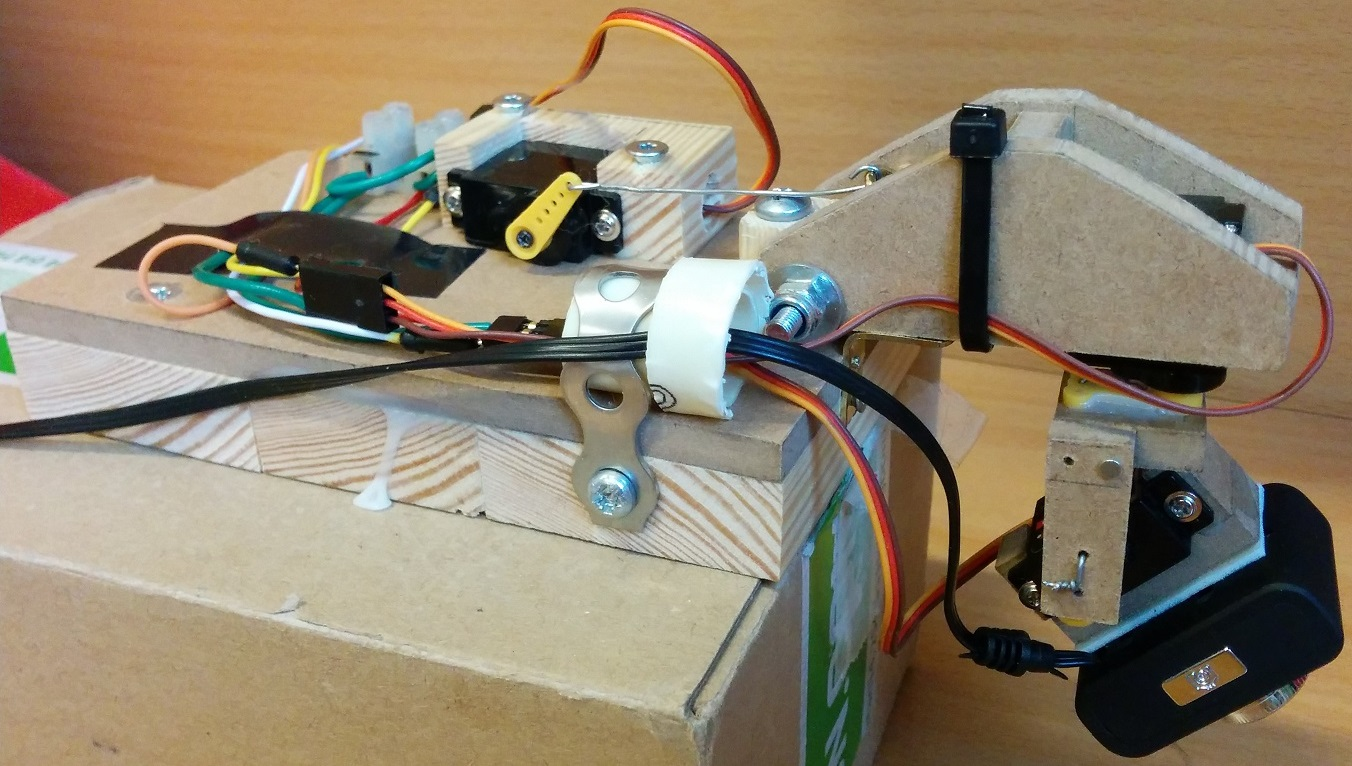
\includegraphics[scale=0.25]{img/Rigg_Bilde.jpg}
	\caption{Prototyperigg}
	\label{fig:RiggBilde}
\end{figure}

Servomotorene styres av et PWM signal som genereres av en Arduino UNO. Biblioteket $Servo.lib$ brukes for å kontrollere servoene gjennom tre I/O porter. Servo 1 er koblet til port 9, servo 2 er koblet til port 6 og servo 3 er koblet til port 3. Siden det viste seg ved målinger at hver servo, under last, kan trekke opp mot 250mA, ble det valgt å bruke en ekstern 6V batteripakke, med fire seriekoblede 1.5V AA batterier, koblet inn som vist i figur [\ref{fig:ArduSkjem}]. Dette isteden for å la servoene trekke forsyningsstrøm rett fra 5V pinnen til arduinokortet. Arduinokortet bruker strøm fra USB og denne kan ikke levere mer enn 500mA ,på grunn av innebygget sikring i Arduino. Dermed kan ikke Arduinokortet levere de ca. 750mA som trengs dersom alle servoene går med stor last samtidig. 

\begin{figure}[h!]
	\centering
	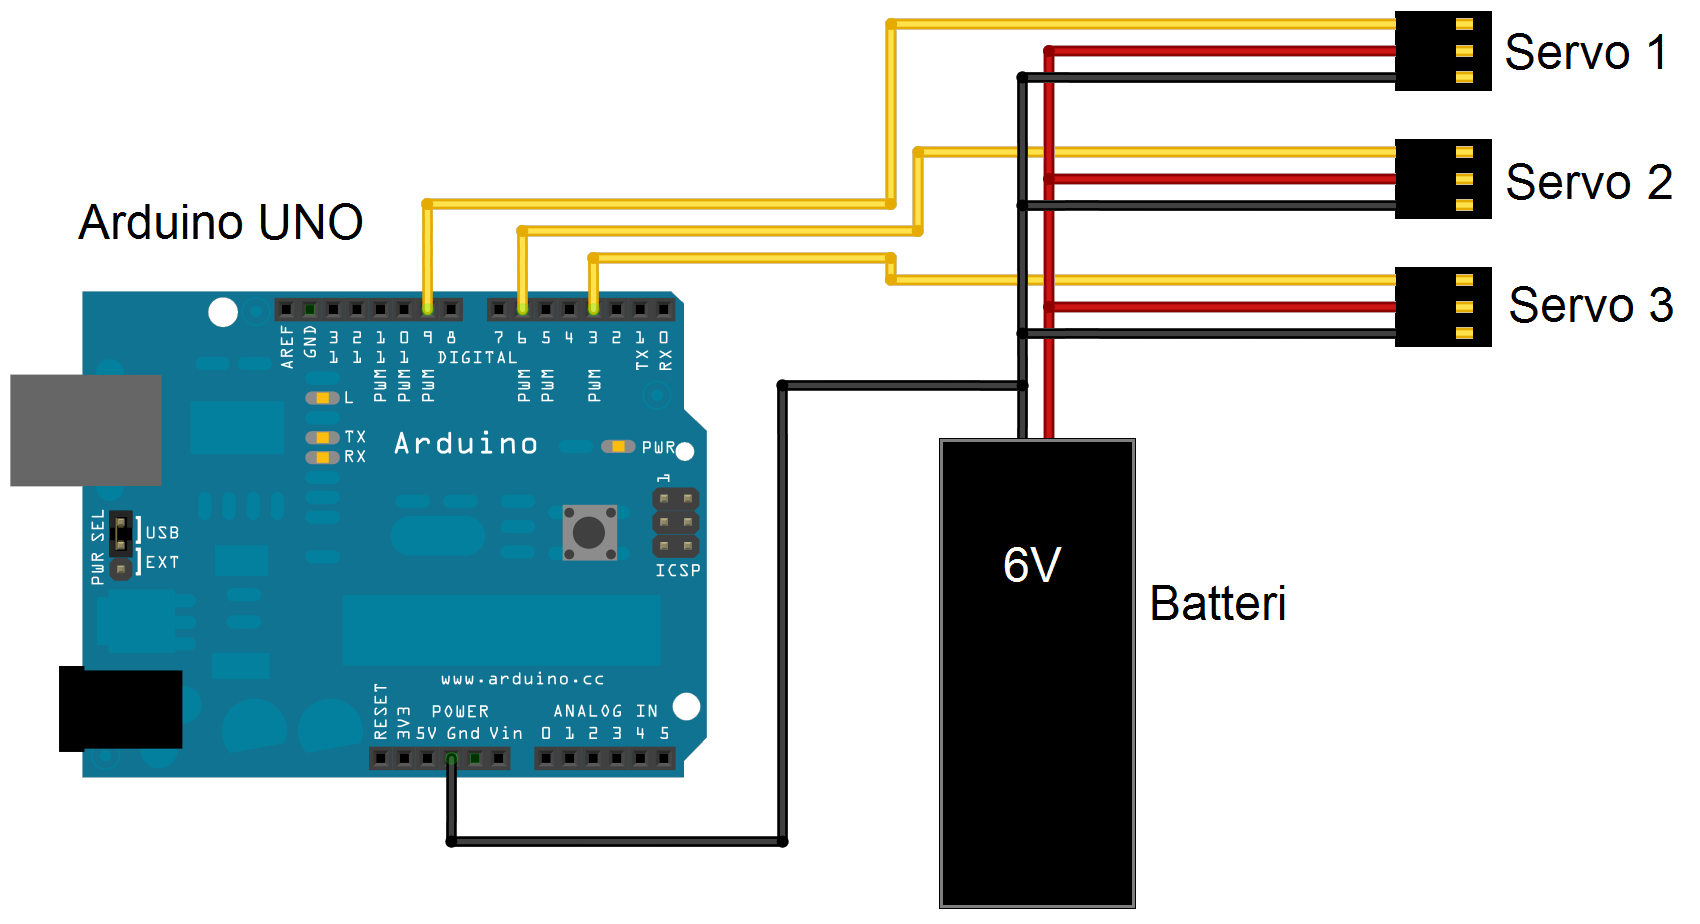
\includegraphics[scale=0.25]{img/KoblingsskjemaArduino.png}
	\caption{Koblingsskjema for Arduino}
	\label{fig:ArduSkjem}
\end{figure}  

Kommandoer sendes til Arduino via USB porten. Kommandoer kan sendes som $Char$ på formen ``100a120b40c'', hvor tallene foran``c'' forteller posisjon til servo 1, tallene for ``b'' gir posisjon til servo 2 og tallene foran ``c'' posisjonenen til servo 3. Dermed vil strengen ``100a120b40c'' flytte servo 1 til 100 grader, servo 2 til 120 grader og servo 3 til 40 grader. De gyldige vinklene er fra 0 til 180 grader. Hvis ``200'' sendes vil servo 1 stoppe på 180 grader. 


\subsection{Styring av rigg + bildegjenkjenning}

Tekst her
